\documentclass{uai2025} % for initial submission
%\documentclass[accepted]{uai2025} % after acceptance, for a revised version; 
% also before submission to see how the non-anonymous paper would look like 
                        
%% There is a class option to choose the math font
% \documentclass[mathfont=ptmx]{uai2025} % ptmx math instead of Computer
                                         % Modern (has noticeable issues)
% \documentclass[mathfont=newtx]{uai2025} % newtx fonts (improves upon
                                          % ptmx; less tested, no support)
% NOTE: Only keep *one* line above as appropriate, as it will be replaced
%       automatically for papers to be published. Do not make any other
%       change above this note for an accepted version.

%% Choose your variant of English; be consistent
\usepackage[american]{babel}
% \usepackage[british]{babel}

%% Some suggested packages, as needed:
\usepackage{natbib} % has a nice set of citation styles and commands
    \bibliographystyle{plainnat}
    \renewcommand{\bibsection}{\subsubsection*{References}}
\usepackage{mathtools} % amsmath with fixes and additions
% \usepackage{siunitx} % for proper typesetting of numbers and units
\usepackage{booktabs} % commands to create good-looking tables
\usepackage{tikz} % nice language for creating drawings and diagrams

\usepackage{amsmath}
\usepackage{amssymb}
\usepackage{amsthm}
\usepackage{todonotes}
\usepackage{bm}
\usepackage{subcaption}
\usepackage{fancyvrb}
% \usepackage[ruled]{algorithm2e}

\def\ci{\perp\!\!\!\!\!\perp}

\newtheorem{definition}{Definition}
\newtheorem{proposition}{Proposition}
\newtheorem{theorem}{Theorem}

\title{Expert-In-The-Loop Causal Discovery: Iterative Model Refinement Using Expert Knowledge}

% The standard author block has changed for UAI 2025 to provide
% more space for long author lists and allow for complex affiliations
%
% All author information is authomatically removed by the class for the
% anonymous submission version of your paper, so you can already add your
% information below.
%
% Add authors
\author[1]{\href{mailto:<ankur.ankan@ru.nl>?Subject=Your UAI 2025 paper}{Ankur~Ankan}{}}
\author[1]{Johannes~Textor}

% Add affiliations after the authors
\affil[1]{%
    Institute for Computing and Information Sciences\\
    Radboud University\\
    Nijmegen, The Netherlands
}
\begin{document}

\maketitle

\begin{abstract}
% Causal discovery has received significant attention in the Directed Acyclic
% Graphs (DAGs) literature, leading to the development of numerous automated
% algorithms for learning DAGs from data. Despite these advancements, the
% application of these algorithms in applied domains remains limited, with
% researchers often preferring to manually construct DAGs based on their expert
% knowledge. This preference stems due to some practical issues with these
% algorithms such as making obvious mistakes, and outputting Markov Equivalence
% Class (MEC). As a result of these issues users typically have to rely on post
% hoc modifications to the model based on their expertise. Given this reliance on
% manual model modification and construction, we propose an iterative method to
% assist researchers in manually constructing DAGs by combining implied
% Conditional Independence (CI) based model testing and utilizing their expert
% knowledge. We present a novel measure of partial association for mixed data
% that allows us to rank violations of implied CIs in the model. Using this
% ranking users can prioritize modifications to the model while using their
% expert knowledge to decide orientation of edges. Empirically, we show that
% a greedy approach achieves performance comparable to automated algorithms, provided
% the user can correctly determine the edge orientation in $ 1 $ out of $ 3 $ cases.
% Additionally, we show that in the absence of an expert, a Large Language Model can
% potentially be used for determining edge orientations.

Causal discovery has received significant attention in the Directed Acyclic
Graphs (DAGs) literature, leading to the development of numerous automated
algorithms for learning DAGs from data. However, their adoption in applied
domains remains limited, as researchers often prefer to construct DAGs manually
based on their expert knowledge. This preference arises due to several
practical issues with these automated algorithms, such as making obvious errors
and outputting Markov Equivalence Classes (MECs). To address these challenges,
we propose an iterative method to assist researchers in manually constructing
or modifying DAGs by combining implied Conditional Independence (CI) testing
with expert knowledge. We introduce a novel measure of partial association for
mixed data to rank violations of implied CIs, enabling users to prioritize
model modifications while leveraging their expertise to decide the orientation
of edges when making these modifications. Empirical results show that this
approach achieves performance comparable to automated algorithms, assuming the
user can correctly orient edges in one out of three cases. Additionally, we
demonstrate that, in the absence of an expert, a Large Language Model can
potentially determine edge orientations.

\end{abstract}

\section{Introduction}
Understanding cause-and-effect relationships between variables is a fundamental
objective in many scientific fields. These relationships reveal the mechanisms
behind observed phenomena and guide effective interventions or policy
decisions. \emph{Causal Discovery} methods aim to discover such relationships
among random variables using observational data. Approaches to causal discovery
have been developed within both the Directed Acyclic Graphs (DAGs) and
Structural Equation Models (SEMs) frameworks, each adapting a different
approach.

In the DAG literature, the primary focus has been on developing automated
algorithms to learn causal structures from datasets. These efforts have led to
numerous causal discovery algorithms, including constraint-based methods like
the PC algorithm \citep{Spirtes2001} and Fast Causal Inference (FCI)
\citep{Spirtes2000}), score-based methods such as Hill-Climb Search and Greedy
Equivalence Search (GES) \citep{Chickering2002}, and continuous
optimization-based methods like NO TEARS \citep{Zheng2018} and DAGMA
\citep{Bello2022}. In contrast, the SEM literature has focused on developing
tools to assist researchers in manually constructing or modifying models,
enabling experts to incorporate their domain knowledge in the model building
process. Researchers typically begin with an initial model based on their
expertise and then use these tools to guide modifications that improve the
model's fit to data. This process is commonly known as \emph{Specification
Search} \citep{Long1983} and uses method such as modification indices, and
Wald-based tests \citep{Marcoulides2018}. While there has been some effort in
DAG literature as well towards allowing for expert knowledge but these methods
focus towards providing the expert knowledge to the automated algorithms
\citep{Bang2023, Meek1995}. \todo[inline]{Whether to keep this sentence?}

Despite the availability of many automated algorithms for constructing DAGs,
their adoption in applied research remains limited. Researchers often prefer to
manually construct DAGs based on their domain expertise \citep{Tennant2020,
Petersen2021}. We believe this preference persists due to several challenges
with these algorithms when applied in practical settings:

\begin{enumerate}
	\item \textbf{Lack of Trust:} While most algorithms are
		asymptotically consistent, their finite sample properties are
		not well understood \todo{Is there any citation for this}.
		Additionally, their output can vary significantly depending on
		the chosen algorithm and their hyperparameters. Combined with a
		lack of robust methods to test these algorithms' performance on
		a given dataset, it can be difficult to trust their outputs. As
		a result, even when using these algorithms are used,
		researchers often rely on post hoc manual modifications to the
		model based on model testing and their domain expertise.
	\item \textbf{Outputs Markov Equivalence Class (MEC):} As multiple
		DAGs can be faithful to a given observational dataset, the
		algorithms can only recover the MECs. These MECs can contain a
		combination of directed and undirected edges. However, most
		methods for downstream tasks, such as identification or causal
		effect estimation, assume knowledge of a fully oriented DAG. As
		a result, researchers have to manually orient these edges based
		on their expert knowledge before using them for analysis.
\end{enumerate}

Fig.~\ref{fig:intro} highlights some of these issues using the Adult income
dataset \citep{Becker1996}. As can be seen in the figure depending on the
sample size and the algorithm used, we get vastly different results.

As a result of these challenges users have relied on model testing approaches
along with their expert knowledge to construct these models. The other ways is
to do post hoc modification to the learned model using implied CI based model
testing \citep{Ankan2021, Ankan2023}. In this testing procedure, users test
whether the implied CIs of the DAG hold in the dataset or not using statistical
CI tests. Based on the results of these statistical tests, we can accordingly
make modifications to the current model to fix the violations. However, this CI
based testing also has a few drawbacks: 1) CIs are implied only by missing
edges in the model, so we can not test for already existing edges. 2) In high
sample size scenarios, p-values can suggest a significant association between
variables even if they have a very weak relationship. 3) Number of implied CIs
can be large making it difficult to manually go through each of them; for
example, in the moderately sized alarm network with $ 37 $ node, there are
$287$ implied CIs. 

There has been work on integrating expert knowledge into model building process
and has been quite successful such as tpc and background knowledge
specification. There has been work on trying to come up with a single test to
combine all these test to give a single answer \citep{Eulig2023, Shipley2000}.
However, what is missing is the guide on how to how to fix these tests.
Additionally there has been a lot of work to integrate expert knowledge into
causal discovery algorithms which has shown significant improvement. To tackle
these issues with CI based testing, we take inspiration from \emph{modification
indices} in specification search. The modification indices method tries to
identify and rank changes in the model such that modifications that improve the
model fit the most are ranked higher.This ranking allows researchers to focus
first on the suggestions that can improve the model the most and while
integrating their expertise to choose the most optimal modifications. Analogous
to this, in this paper we develop a measure for partial association for mixed
data that allows us to rank the CI violations. Additionally, this measure of
conditional association also allows us tackle other issues with CI based
testing outlined in the previous paragraphs.

\begin{figure}
\begin{subfigure}{0.25 \textwidth}
	\includegraphics[page=1]{figures.pdf}
	\caption{PC algorithm $ \chi^2 $ test. $ N=400$ }
\end{subfigure}%
\begin{subfigure}{0.25 \textwidth}
	\includegraphics[page=2]{figures.pdf}
	\caption{PC algorithm $ \chi^2 $ test. $ N=800$ }
\end{subfigure}
\begin{subfigure}{0.25 \textwidth}
	\includegraphics[page=5]{figures.pdf}
	\caption{Hill Climb Search BIC Score. $ N=400$ }
\end{subfigure}%
\begin{subfigure}{0.25\textwidth}
	\includegraphics[page=6]{figures.pdf}
	\caption{Hill Climb Search BIC Score. $ N=800$ }
\begin{subfigure}{0.25 \textwidth}
	\includegraphics[page=3]{figures.pdf}
	\caption{PC algorithm residualization test. $ N=400$ }
\end{subfigure}%
\begin{subfigure}{0.25\textwidth}
	\includegraphics[page=4]{figures.pdf}
	\caption{PC algorithm residualization test. $ N=800$ }
\end{subfigure}
\end{subfigure}

\caption{Markov Equivalence Class (MEC) learned for Adult Income Dataset using (a) PC algorithm with chi-squared test, (b) Hill-Climb Search with BIC score, (c) PC algorithm with residualization based test. There is significant variation in the learned model depending on the sample size and the algorithm used. Additionally, all of them make some mistakes.}
\label{fig:intro}
\end{figure}

Our main contributions in this paper are as follows:
\begin{enumerate}
	\item We present a measure of (conditional) association for mixed data
		based on canonical correlations. This measure of association
		generalizes the widely used partial correlation to mixed data
		setting.
	\item Using this partial association measure, we present a procedure to
		rank CI tests. This ranking can be used to prioritize addition
		or deletion of edges from the model.
	\item We present both a web-browser based tool and an implementation in
		the Python package to allow researchers to apply this method to
		their own datasets.
\end{enumerate}

The rest of the paper is structured as follows. In
Section~\ref{sec:background}, we give a background on the measures of
association for various data types. In Section~\ref{sec:mixed_association}, we
present our method for computing mixed data association. In
Section~\ref{sec:modification} and Section~\ref{sec:web}, we present how to use
this method to make modifications and the web tool, and lastly in
Section~\ref{sec:empirical}, we show some empirical analysis on how well this
modification process works.

\section{Background and Related Work}
\label{sec:background}
\subsection{Notations}
We consider random variables $ X $ and $ Y $ with a possible multi-dimensional
variable $ \bm{Z} = \{ Z_1, \cdots, Z_k \} $. We consider these variables in
the mixed data setting where these variables can be any combination of
continuous, categorical, or ordinal unless specified. We also assume all
variables to be observed. We use $ \rvert \bm{Z} \rvert $ to represent the
cardinality of the variable $ \bm{Z} $. We write $ \bm{x} = (x_1, \cdots, x_n)
$ for a sample from $ X $ of size $ n $. We write the expectation of a variable
$ X $ as $ \mathbb{E}[X] $, conditional expectations as $ \mathbb{E}[X |
\bm{Z}] $.

We consider the problem of estimating the partial (or conditional) association
between $ X $ and $ Y $ in the presence of a set of conditioning variables $
\bm{Z} $. When $ Z = \emptyset $, this is equivalent to the marginal
association between $ X $ and $ Y $.

\subsection{Measures of Conditional Association}
As our DAG construction procedure relies on a measure of conditional
association between variables, in this section we list out some of the already
known measures for specific data types. These measure of associations are
typically the effect size of various conditional independence tests but they
don't need to be. However, there are no generalized measure of association for
mixed data, that we propose in the next section. This is by no means an
exhaustive list, rather just to give an idea of what can be done.

\paragraph{Both $ X $ and $ Y $ are continuous}
Where there are no conditional variables, $ \bm{Z} = \emptyset $, Pearson's
correlation coefficient can be used as a measure of association between the
variables. This does make various assumptions such as linearity between the
variables, normal distribution for $ X $ and $ Y $, and homoscedasticity.

In the case when $ \bm{Z} \neq \emptyset $, then partial correlations can be
used. This requires using two linear regression models: $ E_X: X \sim \bm{Z} $
and $ E_Y: Y \sim \bm{Z} $. Then computing the residuals using these two
regressions as: $ R_X = X - E_X(\bm{Z}) $ and $ R_Y = Y - E_Y(\bm{Y}) $. After
this a simple correlation coefficient can be computed between $ R_X $ and $ R_Y $.

\paragraph{All $ X $, $ Y $, and $ \bm{Z} $ are discrete}

In the case of discrete variables, Cramer\'s V has been typically used as a
measure of association. When there are no conditional variables, $ \bm{Z} =
\emptyset $, Cramer\'s V can be computed directly from the contingency table.

However, when conditional variables are present, we can iterate over all
possible combinations of the conditional variables, compute the Cramer\'s V and
then lastly combine them together. 

\paragraph{$ X $ is ordinal and $ Y $ is continuous or ordinal}
Polyserial Correlation (when one is oridinal and the other is continuous) and
polychoric correlation (when both are ordinal) can be use. Here the assumption
is made that $ X $ is a thresholded version of an underlying continuous normal
variable. The method then tries to learn the thresholds for this latent
variable while trying to maximize the correlation between $ X_{lat} $ and $ Y
$. This gives us values that are Pearson's correlation coefficient.

\section{A Measure of Association for Mixed Data}
\label{sec:mixed_association}

In this section, we introduce a novel measure of partial association for mixed
data by extending the concept of partial correlations \citep{Whittaker2009}
\todo{Verify this citation} to handle mixed data types. To compute partial
correlations, we have two key steps: 1) a residualization method, and 2) a
measure of associations between the residuals. When both $ X $ and $ Y $ are
continuous variables, residuals are typically computed using a regression-based
method, and Pearson's correlation coefficient is used to measure the association
between these residuals. To extend this approach to mixed data, we combine a mixed
data residualization method \citep{Ankan2023} with a multivariate measure of
association based on canonical correlations, Pillai's Trace \citep{Pillai1955}. 

Given $ n $ samples $ D = (x, y, \bm{z}) $ of variables $ X $, $ Y $, and $
\bm{Z} $, we aim to estimate the conditional
association $ \rho(X, Y; \bm{Z}) $ between $ X $ and $ Y $ conditioned on $
\bm{Z} $. We use the residualization approach from \citet{Ankan2023} to compute 
the residuals. The residuals are defined as follows, depending on the type of 
dependent variable:

\begin{enumerate}
	\item \textbf{Continuous:} We train a regression model, $ E_X: x \sim
		\bm{z} $. The residuals are then defined as the difference
		between the true and the predicted values using $ E_X $. 
		$$ R_{x_i} = x_i - E_X(\bm{z}_i) $$
	\item \textbf{Ordinal:} We start by training a probability estimator, $
		p_X: x \sim \bm{z} $, and obtain probability predictions 
		$ \hat{p}_X: \hat{p}_X(\bm{Z}) $. Then, we compute the residuals
		as follows \citep{Li2012}:
		$$ R_{x_i} = \hat{p}(\hat{x}_i > x_i) - \hat{p}(\hat{x}_i < x_i) $$
	\item \textbf{Categorical:} We again start by training a probability
		estimator $ p_X: X \sim \bm{Z} $, and obtain probability
		estimates $ \hat{p}_X: p_Z(\bm{Z}) $. Next, we dummy encode the
		categorical variable and then compute the residuals as follows: 
		$$ R_X = x_i - \hat{p}(\bm{z}_i) $$
\end{enumerate}

\todo[inline]{Fix notations above}

We repeat the above step for the variable $ Y $ and compute its residual $ R_Y
$. Here, we have the option to choose the estimators based on the properties of
the data. Non-parametric ensemble estimators such as Random Forest and XGBoost
can handle any combination of data types while performing reasonably well. For
linear datasets, we can also choose variants of linear regression depending on
the type of data. 

After the above steps are repeated for both $ X $ and $ Y $, we end up with two
residual matrices: $ R_X $ and $ R_Y $. The type of the variable determines the
shape for these matrices. If the variable is continuous, we get a residual
matrix of shape $ ( n \times 1 ) $ and if the variable is categorical, we have
a residual matrix of shape $ ( x \times (k -1)) $ where one of the dummy encoded
variables is dropped to avoid multicollinearity.

We now have two continuous-valued residual matrices. The next step is
to quantify the association between these residuals. In multivariate
statistics, canonical correlation based measures have been used to measure
the association between two sets of variables. We can treat our residuals
as sets of variables and use canonical correlations to quantify the association
between them.

\begin{definition} 

	Given two sets of random variables $ \bm{U} = (U_1, U_2, \cdots, U_p) $
	and $ \bm{V} = (V_1, V_2, \cdots, V_q) $, canonical correlation between
	them, $\rho(\bm{U}, \bm{V}) $ is defined as:
		
	% \begin{equation}
	% 	\phi(\bm{U}, \bm{V}) = \sup_{a, b} \frac{a^T \Sigma_{\bm{U}\bm{V}} b}{\sqrt{a^T \Sigma_{\bm{U}\bm{U}} a} \sqrt{b^T \Sigma_{\bm{V}\bm{V}} b}}
	% \end{equation}

% \begin{equation}
% 	\begin{split}
% 		\bm{\rho}(\bm{U}, \bm{V}) &= \sqrt{\mathrm{E} \left( \Sigma_{\bm{UU}}^{-1} \Sigma_{\bm{UV}} \Sigma_{\bm{VV}}^{-1} \Sigma_{\bm{VU}} \right)}
% 	\end{split}
% \end{equation}
	\begin{equation}
		\rho(\bm{U}, \bm{V}) = \max_{a, b} Corr(a^T \bm{U}, b^T \bm{V})
	\end{equation}

	where $ a $ and $ b $ are vectors of coefficients that maximize the correlations
	between the linear combinations of $ a^T \bm{U} $ and $ b^T \bm{V} $.
\end{definition}

% where $ \mathrm{E}(\Sigma) $ denotes the eigenvalues of the matrix $ \Sigma $.
% $ \Sigma_{UU} $ and $ \Sigma_{VV} $ are the covariance matrices of $ \bm{U} $
% and $ \bm{V} $, and $ \Sigma_{UV} $ and $ \Sigma_{VU} $ are the
% cross-covariance matrices.
	
Canonical correlations generalize correlations to multi-dimensional variables. They
find orthogonal linear transformations $ a $ and $ b $ of $ \bm{U} $ and $ \bm{V} $
such that the correlation between the transformed variables $ a^T \bm{U} $ and 
$ b^T \bm{V} $ is maximized. This yields a vector of correlation values of 
size $ \min(p, q) $, representing the correlation coefficient of each pair of 
transformed variables. Pearson's correlation coefficient is a special case of 
canonical correlations when $ p = q = 1 $.

Many measures of association based on canonical correlation have been used in
multivariate statistics, each with slightly different properties.
\begin{itemize}
	\item Wilks' Lambda:
		$$ \Lambda = \prod_{i}^{\min(p, q)} (1 - \phi_i^2) $$
	\item Roy's Largest Root: 
		$$ \theta = \max_i(\phi_i^2) $$
	\item Pillai's Trace: 
		$$ \tau = \sum_{i=1}^{\min(p, q)} \phi_i^2 $$
\end{itemize}

We use Pillai's Trace for our purpose for two main reasons: 1) It uses all the
canonical correlation values, 2) Its interpretation is similar to correlation
coefficient, i.e., $ 0 $ signifies no association and $ 1 $ signifies perfect
linear relationship. This gives us the following partial measure of
association:

\begin{equation}
	\rho(X, Y; \bm{Z}) = \frac{1}{\min(\rvert R_X \rvert, \rvert R_Y \rvert)}
	\sum_{i=1}^{\min(\rvert R_X \rvert, \rvert R_Y \rvert)} (\phi_i(R_X, R_Y))^2
\end{equation}

This measure of association has many desired properties:

\begin{enumerate}
	\item \textbf{Bounded: } $ \rho $ is bounded between $ 0 $ and $ 1 $,
		with $ 0 $ representing no association while $ 1 $ represents
		perfect linear association. This helps in interpretation and
		comparing values across multiple partial associations.
	\item \textbf{Independent of Sample Size: } The measure remains consistent
		regardless of the sample size ensuring reliability across 
		studies with different sample sizes.
	\item \textbf{Invariant to the Dummy Encoding Scheme: } Since canonical
		correlations search for linear combinations over the columns,
		the measure is invariant to the specific dummy encoding
		scheme used for categorical variables.
	\item \textbf{Generalizes Partial Correlations to Mixed Data: }
		Canonical correlations is equivalent to Pearson's correlation coefficient
		when both $ X $ and $ Y $ are continuous. Hence, $ \rho $ generalizes
		partial correlations to mixed data types.
	\item \textbf{Related to Cramer\'s V: } 
\end{enumerate}

So, in a sense this measure generalized currently used measures of associations
to mixed data.

\section{Using Measure of Association for DAG Modification and Construction}
\label{sec:modification}

Using this mixed data partial association measure, we propose a method to rank
CI tests, and use it for model construction and modification. Given a
potentially empty DAG $ G $ and a dataset $ D $, for each pair for variable $ X
$ and $ Y $ in $ G $:
\begin{itemize}
	\item If there is no edge between $ X $ and $ Y $, we compute p-value for the CI test $ X \ci Y \rvert pa_G(X) \cup pa_G(Y) $ and the partial association measure: $ \rho(X, Y; pa_G(X) \cup pa_G(Y)) $.
	\item If there is an edge between $ X $ and $ Y $, we compute p-value for the CI test $ X \ci Y \rvert pa_{\underline{G}}(X) \cup pa_{\underline{G}}(Y) $ and the partial association measure: $ \rho(X, Y; pa_{\underline{G}}(X) \cup pa_{\underline{G}}(Y) $.
\end{itemize}

For a pair of variables $ X $ and $ Y $, if there is an edge present between
them, the interpretation of this partial association measure is similar to path
coefficients in SEMs, i.e. how strong is the edge between the variables. Hence,
we can use this to identify potential edges that can be removed from the model.
In the case when there is no edge between the variables, the value of this
partial measure of association can be interpreted as - given the current
structure of the model how much of the observed correlation between the
variables $ X $ and $ Y $ in data is not explained by the model. To modify the
model based on this, we can look at the pair of variables that have an edge
between them. If any of these pair have a p-value greater than partial
association below our chosen threshold, we can remove that edge as it is
redundant.

The measure of association also gives us a way to rank the potential
modifications. The smallest values (below the threshold) of the association
measure are the worst offending ones and for when the edges are not present the
largest values would add the most amount of explainability to the model. Using
this ranking the user can decide which pair of variables to focus on.

We can then use this to rank pair of variables which have very high unexplained
association between them. Based on the domain expertise, we can then choose one
of these suggested pair of variables, decide the direction of the edge between
the variables, and add it to the model. Once the new edge is added we can
recompute the association of all other variables and $ X $ and $ Y $.

Additionally, in each iteration of modification, for each pair of variable in $
G $, that has an edge between them in we compute the partial association
measure: $ \rho(X, Y; pa_{\underline{G}}(X) \cup pa_{\underline{G}}(Y) $. This
measure of association can be interpreted as the strength of the edge between
the variables. If the value of this association below a certain threshold, we
can remove the edge.

\todo[inline]{Add a figure showing an example of how this modification works.}

\begin{theorem}
	If we have access to an oracle that can give correct edge directions, taking a
	greedy approach with the procedure above results in the correct graph
	being recovered. \todo[inline]{Reword and add proof}
\end{theorem}

\section{Connection to Score Based Methods}
\begin{itemize}
	\item The process of iteratively adding and removing edges in very similar to
		Greedy Equivalence Search (GES).
	\item But not decomposible like scoring methods. 
	\item But Because they make only local changes, can get stuck in local minimas.
	\item Both approach looks for modifications globally.
	\item The sum of unexplained effect provides an absolute measure of model fit 
		unlike scoring methods.
\end{itemize}

\section{Web Tool}
\label{sec:web}
Based on the procedure outlined in the previous section, we built a web-based
tool that allows us to interactively create/modify their model. The user
starts by uploading their dataset and optionally the initial DAG. If no initial
DAG is provided an empty graph is initialized. The tool also computes the
Shipley's C value at any point. The web-tool would automatically show all
unexplained associations in the DAG by adding red edges between them. The edge
weight of the edge represents how high this strength is. Users can also set the
threshold for p-value and association to control how many edges are shown at a
time. Based on these shown potential edges, the user can select the edge that
they want to add and decide the direction for it. If the tool detects an
incorrect edge in the graph, it is shown in black. Once the user is happy with
the graph they have they can export it into different formats to use it for
further computation.

\begin{figure}
	\centering
	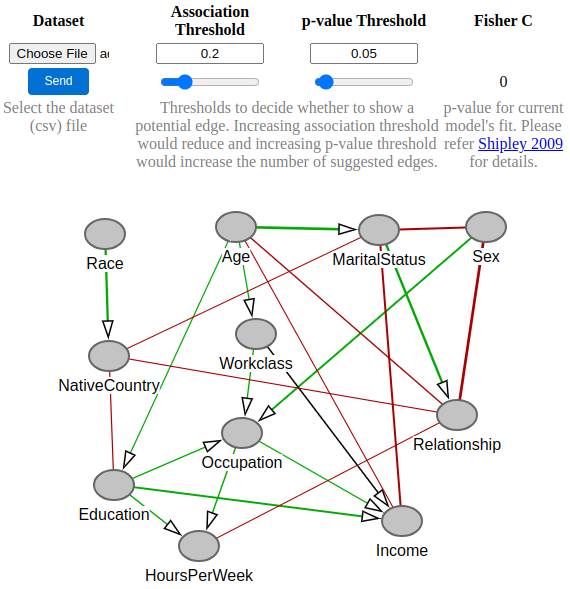
\includegraphics[scale=0.4]{../code/plots/web_tool_full.png}
	\caption{A screenshot of the web tool for constructing the model. Users
		can upload their dataset after which the tool creates an empty
		graph and shows all pair of variables which are associated in
		the model using undirected red edges with the strength of
		association represented using edge width. Users can then add
		edges to the model (shown in green). Unnecessary edges are shown in 
		black.}
\end{figure}

% \begin{figure}
% 	\centering
% 	\begin{subfigure}{0.5\textwidth}
% 		\includegraphics[scale=0.25]{../../presentations/2024_05_das/2.png}
% 	\end{subfigure}%
% 	\begin{subfigure}{0.5\textwidth}
% 		\includegraphics[scale=0.25]{../../presentations/2024_05_das/5.png}
% 	\end{subfigure}
% 	\caption{Screenshots of the web-tool. \todo[inline]{Insert screenshots of the web-tool}}
% \end{figure}

\section{Empirical Analysis}
\label{sec:empirical}

\begin{figure}
	\centering
	\begin{subfigure}{0.5\textwidth}
		\centering
		\includegraphics{../code/fig3/shd_ribbon.pdf}
		\caption{}
	\end{subfigure}
	\begin{subfigure}{0.5\textwidth}
		\centering
		\includegraphics{../code/fig3/sid_ribbon.pdf}
		\caption{}
	\end{subfigure}
	\caption{Comparison of PC and Hill-Climb Search algorithms against
		manually drawn DAGs using the assistance method. As PC and
		Hill-Climb Search return the Markov Equivalence Class (MEC), we
		use the best and worst scoring orientation of the MEC to get
		the range of values. The human drawn values are done for
		multiple accuracy values of the oracle.}
\end{figure}

\begin{figure}
	\begin{subfigure}{0.25\textwidth}
		\centering
		\includegraphics{../code/fig4/unexplained_effect.pdf}
		\caption{}
	\end{subfigure}%
	\begin{subfigure}{0.25\textwidth}
		\centering
		\includegraphics{../code/fig4/ll.pdf}
		\caption{}
	\end{subfigure}
	\caption{Plots showing improvements in fit of the model over iterations
	on the Adult income dataset. For the expert simulation an LLM is used
	for the edge orientations. (a) Shows using total unexplained effect that is the
	sum of effect size between variables that don't have an edge between them. (b)
	Shows the log-likelihood of the overall model.
	}
\end{figure}

We analyzed the performance of this manual approach by comparing it with two
automated algorithms: PC and Greedy Equivalence Search (GES). For the
comparison we use simulated data from a known DAG and compare how well the
algorithm is able to recover the original model using two metrics: Structural
Hamming Distance (SHD) and Structural Intervention Distance (SID). To simulate
the data, we start with a randomly generated DAG on $ 10 $ nodes and use linear
models with random effects to generate the data. 

We vary the edge probability of the DAG to generate DAGs with varying density.
We repeat the data generation $ 30 $ times for each density value for the DAG.
As both PC and Hill-Climb Search can only give us a CPDAG, we compare the
orientation of these CPDAG which result in the best and worst case scores on
SHD and SID.

To use our proposed approach, we need an expert to tell us the direction of the
edges. We simulated an expert using this assisted model construction approach,
we start with an empty model and take a greedy approach to add edges to this
model. At any point, we select the pair of variables that has significant
correlation and the highest unexplained correlation, i.e., highest conditional
association. We then use an oracle to decide the direction of the edge between
the variables. Given an accuracy of the oracle, $ \alpha $, the oracle either
gives the correct direction, incorrect direction, or returns None representing
that it does not know the direction.

\begin{equation}
	\begin{split}
		x &= \textnormal{rand}([0, 1]) \\
		O(\alpha) &= \begin{cases} 
			M \rightarrow Y, & \textnormal{if  } x <= \alpha \\
			\textnormal{rand}(M \rightarrow Y, M \leftarrow Y, None) & \textnormal{otherwise} \\
				\end{cases} \\
	\end{split}
\end{equation}

If the oracle returns None for any pair of variables, an edge between this pair
is not suggested to the oracle in future iterations. We also make sure that
only edges which do not form a cyclic in the graph are used to select the next
potential edge. After adding each edge, we also check if the p-value of any
existing edge shows independence. If that happens we remove that edge and
blacklist that edge, i.e., that edge is not prompted again during the run of
the algorithm. We repeat this procedure till the model explains all
correlations between the variables. There is a possibility that this greedy
expert gets stuck at incorrect graph structures as it does not do any
backtracking to fix its earlier mistakes. This procedure is outlined in the
Algorithm 1.
\todo[inline]{Show an algorithm of how this expert method is working}

\subsection{Using Large Language Models as Experts}
A lot of recent work has focused on finding pairwise causal direction among
variables using Large Language Models. In this analysis, instead of using the
oracle to decide the direction of edges, we used GPT4 to give us the direction
of the edges based on description of the variables. As GPT4 has already
memorized many of these models, we encoded the variable names using a random
string and provided the description of the variable to let it decide the
direction of the edge.

\begin{figure}
	\centering
	\begin{subfigure}{0.5\textwidth}
		\begin{Verbatim}[fontsize=\footnotesize]
You are an expert in Social Science. Following
are the descriptions of two variables:

<A>: {description of variable A}
<B>: {description of variable B}

Which of the following two options is the most 
likely causal direction between these variables:

1. <A> causes <B>
2. <B> causes <A>

Return a single letter answer between the 
choices above; Do not provide any reasoning 
in the answer; Do not add any text formatting 
to the answer.
		\end{Verbatim}
	\caption{Prompt used for the LLM}
	\end{subfigure}
	\begin{subfigure}{0.5 \textwidth}
		\begin{Verbatim}[fontsize=\footnotesize]
Age: The age of a person
Workclass: The workplace where the person is 
     employed such as Private industry, 
     or self employed
Education: The highest level of education the 
     person has finished
MaritalStatus: The marital status of the person
Occupation: The kind of job the person does. 
     For example, sales, craft repair, clerical.
Relationship: The relationship status of 
     the person
Race: The ethnicity of the person
Sex: The sex or gender of the person
HoursPerWeek: The number of hours per week the 
     person works
NativeCountry: The native country of the person
Income: The income i.e. amount of money the 
     person makes
		\end{Verbatim}
	\caption{Variable descriptions used for prompting the LLM}
	\end{subfigure}
	\begin{subfigure}{0.5\textwidth}
		\centering
		\includegraphics[scale=0.3]{../code/fig5/llm_adult.png}
		\caption{The learned DAG}
	\end{subfigure}
\end{figure}

\section{Conclusions}

\newpage
\bibliography{references}
\end{document}
